\subsection{OSI参照モデル}

インターネットで利用されるプロトコルは、The Internet Engineering Task Force (IETF)という標準化
団体により策定され、その標準はRequest for Comments (RFC)という名のオープンな仕様として発行されている。
例えば、我々が利用しているインターネットプロトコルである
インターネットプロトコル バージョン4は、1981年に791番目のRFCとして策定された~\cite{RFC0791}。

IETF以外の通信に関する標準化団体としては
International Telecommunication Union Telecommunication Standardization Sector (ITU-T)や、
International Organization for Standardization (ISO)が存在する。
実は、1977年から1982年かけて、ITU-TやISOがコンピュータネットワークの標準通信プロトコルとして、
Open Systems Interconnection (OSI)の策定を行っていた。
その当時は標準的な通信プロトコルは存在せず、ベンダーごとに様々なプロトコルが利用されていたため、
通信プロトコルの統一化が求められていたのである。
しかしながら、最終的にOSIは主流とはならず、IETFによって策定された
インターネットプロトコルが広く利用されるようになっていった。

\begin{figure}[tb]
    \centering
    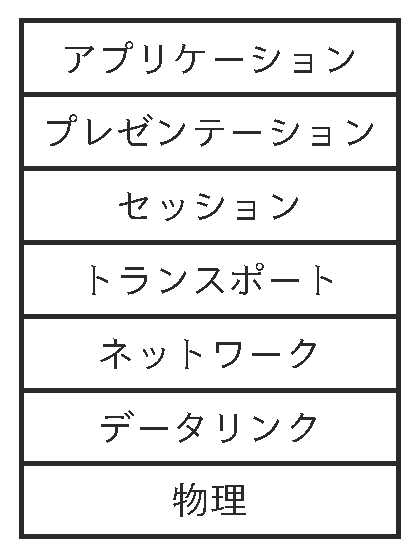
\includegraphics[width=5cm,pagebox=artbox]{figs/OSI.pdf}
    \caption{OSI参照モデル}
    \label{fig:osi}
\end{figure}

OSI自体は残らなかったが、OSI策定の際に考案されたOSI参照モデルと呼ばれる
ネットワークの抽象化手法は、今日でも広く受け入れられている。
図~\ref{fig:osi}は、OSI参照モデルによるネットワークの抽象化モデルを表している。
OSI参照モデルでは、ネットワークの機能を階層構造にもとづいて抽象化しており、
この抽象化をレイヤリングなどと呼ぶ。
OSI参照モデルでは、下から順に1層に物理層、2層にデータリンク層、
3層にネットワーク層、4層にトランスポート層、5層にセッション層、
6層にプレゼンテーション層、7層にアプリケーション層が位置する。
ちなみに、各層のことをレイヤ1、レイヤ2といったり、更に略してL1、L2などということもある。

\begin{figure}[tb]
    \centering
    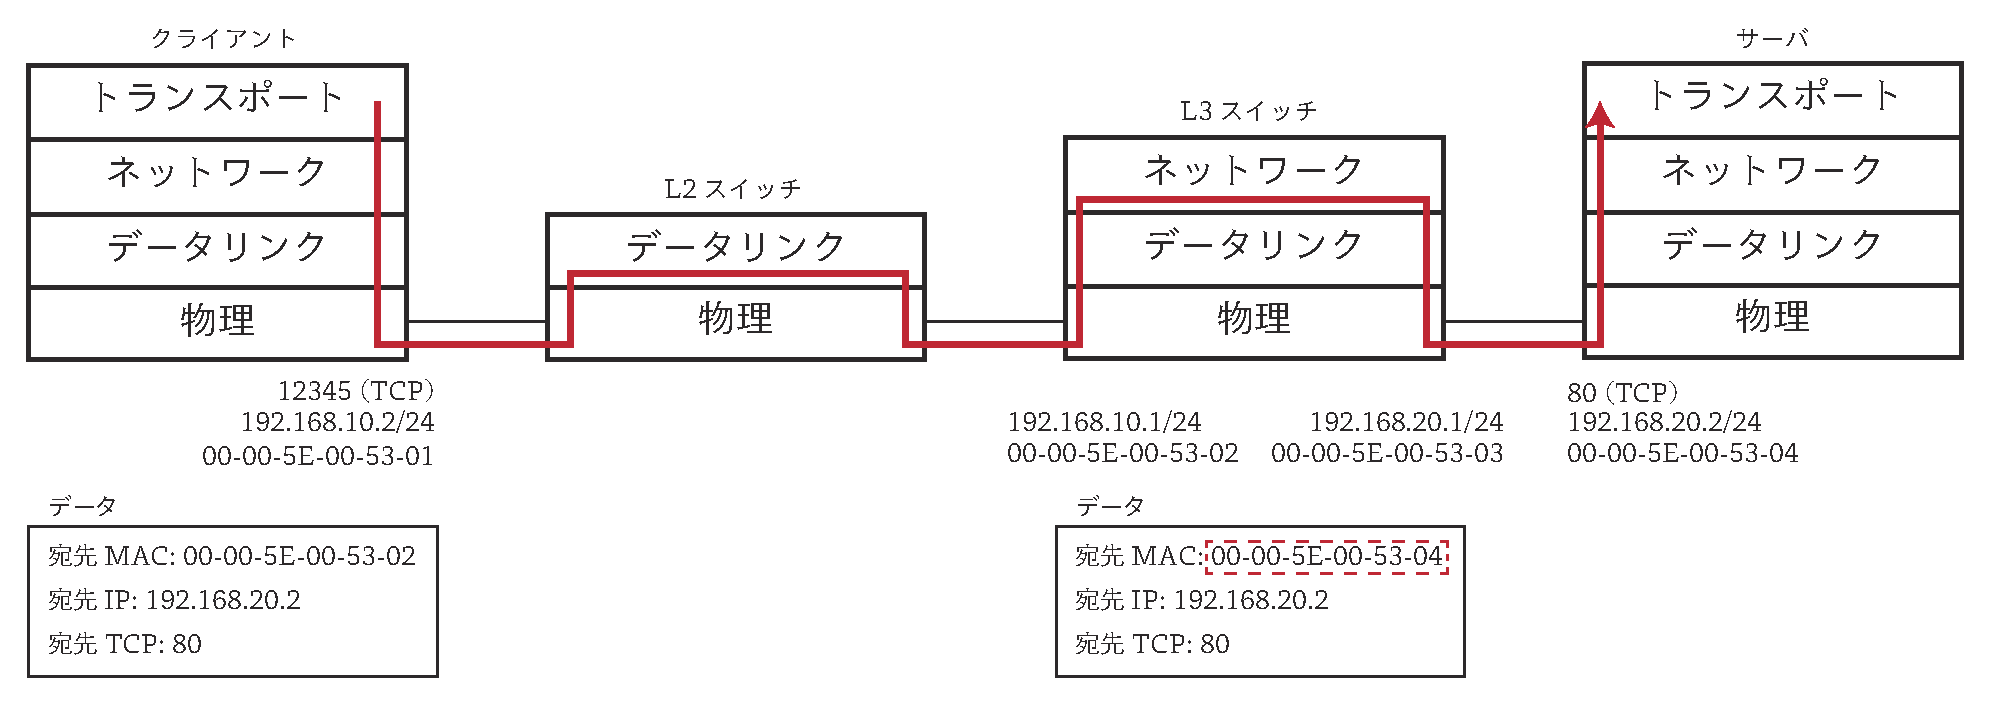
\includegraphics[height=5cm,pagebox=artbox]{figs/osi_link.pdf}
    \caption{各層でのデータ転送}
    \label{fig:osi_link}
\end{figure}

図~\ref{fig:osi_link}は各層でデータ転送が行われている様子を示している。
この図の意味することろを説明するのが本節の目標であるため、
現段階で理解できなくても問題ない。
後ほど振り返る頃には、この図の意味がわかるようになるだろう。

データリンク、ネットワーク、トランスポート層にはそれぞれアドレスがあり、
各層は、そのアドレスに基づいて転送を行う。
データリンク層のアドレスは42ビットで表され、文字で表現すると00-00-5E-00-53-02といった
表記になる。
図~\ref{fig:osi_link}中で宛先MACと示される値は、
データリンク層の宛先MACアドレスを示している。
なお、MACは Media Access Controlの略である。
データリンク層は、ローカルなネットワークでの通信を行うために用いられる。
そのため、MACアドレスはそのローカルな環境では一意に識別できる必要がある。
データリンク層の詳細については~\ref{sec:datalink}節で解説する。

ネットワーク層のアドレスは、192.168.10.2/24で表される32ビットのIPアドレスとなり、
/24はネットワークのサブネット長を示している。
図~\ref{fig:osi_link}では、192.168.10.0/24と192.168.20.0/24
というサブネットが示されている。
ネットワーク層、すなわちIPは、全世界で通信を行うために用いられるプロトコルであり、
基本的にはIPアドレスは世界で一意に識別できるように割り当てるのが設計理念となっている
(現実的にはそうはなっていないが)。
なお、前述のアドレスはIPv4アドレスであるが、IPv6の場合は128ビットのアドレス空間を持つ。
ネットワーク層の詳細については~\ref{sec:network}節で解説する。

トランスポート層のアドレスは16ビットで示され、一般的にポート番号と呼ばれる。
TCPやUDPはポート番号をもとに、アプリケーションの識別を行う。
よく利用されるポート番号は、Well KnownポートTCPの80番ポート

\begin{itembox}[l]{\bf 重要ポイント}
    \begin{itemize}
        \item インターネット関連のプロトコルは、IETFが発行するRFCによって標準化されている
        \item コンピュータネットワークはレイヤで考えることができる
    \end{itemize}
\end{itembox}

\subsection{データリンク層} \label{sec:datalink}

\subsection{ネットワーク層} \label{sec:network}

\subsection{トランスポート層} \label{sec:transport}

\subsection{トランスポートより上の層}